\documentclass{beamer}

\usepackage[utf8]{inputenc} 
\usepackage[T1]{fontenc}
\usepackage{lmodern}
\usepackage{graphicx}
\usepackage[english]{babel}
\usepackage{array}
\usepackage{multirow}
\usepackage{caption}
\usepackage{fixltx2e}
\usepackage{listings}
\usepackage{textcomp}
\usepackage[style=authoryear]{biblatex}

\setbeamertemplate{bibliography item}{[\theenumiv]}

\usetheme{Warsaw}

\bibliography{central-bibliography/bibliography}

\begin{document}


\title{Low-cost IoT, Big Data, and Cloud Platform for Developing Countries}
\author{Corentin Dupont, Tomas Bures, Mehdi Sheikhalishahi, Congduc Pham, Abdur Rahim}		 

\institute{FBK/Create-Net\newline cdupont@fbk.eu}


\maketitle

\begin{frame}
  \frametitle{Table of Contents}
  \tableofcontents[]
\end{frame}


\section{Introduction}
\begin{frame}
\frametitle{Introduction}
  Massive deployment of IoT worlwide \\
  IoT is a great opportunity for developing countries

  \begin{figure}[H]  
  \centering  
  \includegraphics[width=.6\linewidth]{figures/AfricaICTApp}  
  \label{figure-AfricaICTApp}  
  \end{figure}

\end{frame}

\begin{frame}
\frametitle{Introduction}
  
  Difficulties of deployements in Africa:
  \begin{itemize}
    \item lack of infrastructure, 
    \item high cost of hardware
    \item complexity in deployment, 
    \item lack of technological background
  \end{itemize}

  IoT deployment must address:
  \begin{itemize}
    \item Longer range for rural access
    \item Cost of hardware and services
    \item Limit dependancy to proprietary infrastructures
    \item Provide local interaction models
  \end{itemize}

\end{frame}

\begin{frame}
\frametitle{Our contribution}
 
  \begin{itemize}
    \item Low-cost HW with LoRa  
    \item Low-cost Cloud platform for IoT and Big Data
  \end{itemize}

\end{frame}

\section{Entering the IoT era}

\subsection{IoT connectivity}

\begin{frame}
\frametitle{Extreme long-range application with new radio technologies}
Low-Power Wide Area Networks (LoRa):
  \begin{itemize}
    \item 20 kms range LOS
    \item 2-4 kms range non-LOS
    \item single hop
  \end{itemize}



\begin{figure}[H]  
\centering  
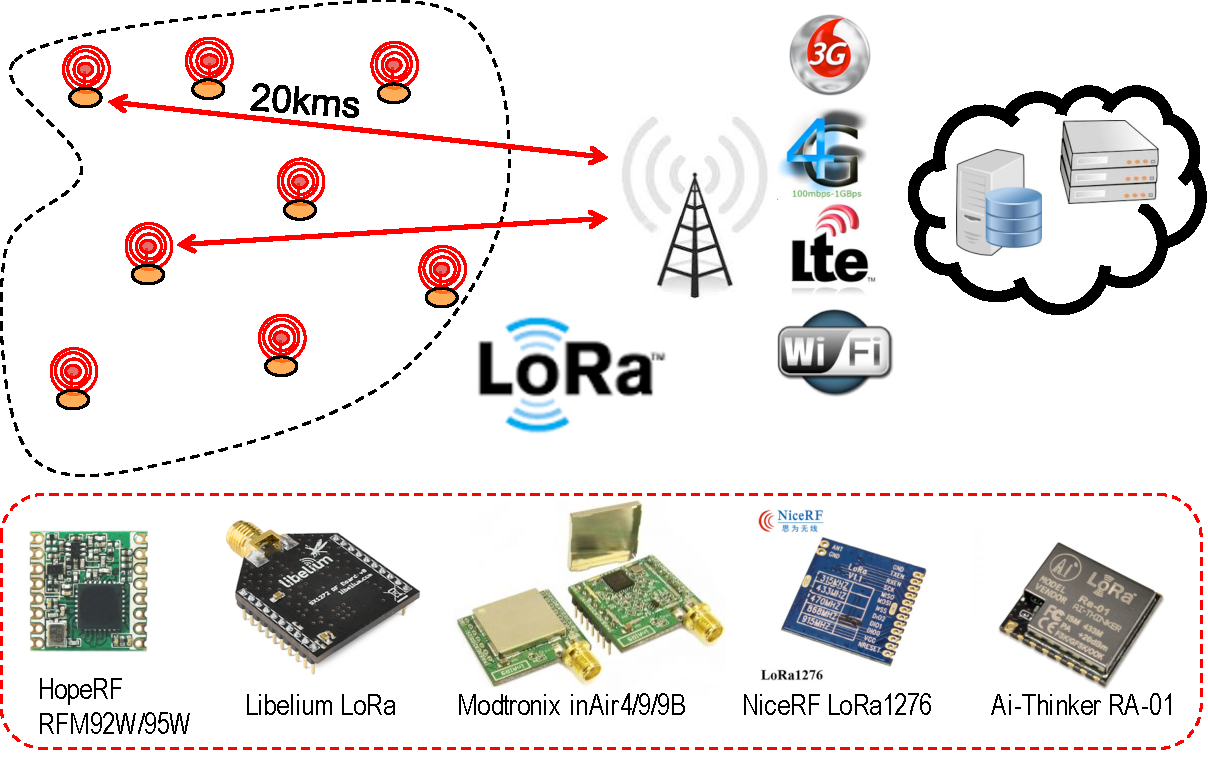
\includegraphics[width=.55\linewidth]{figures/1-hop}   
\label{figure-1hop}  
\end{figure} 
\end{frame}

\subsection{Low-cost DIY IoT hardware}

\begin{frame}
\frametitle{Low-cost DIY IoT hardware}

Gateway: Raspberry-like embedded Linux \\
Sensor nodes: Arduino boards




  \begin{figure}[H]  
  \centering  
  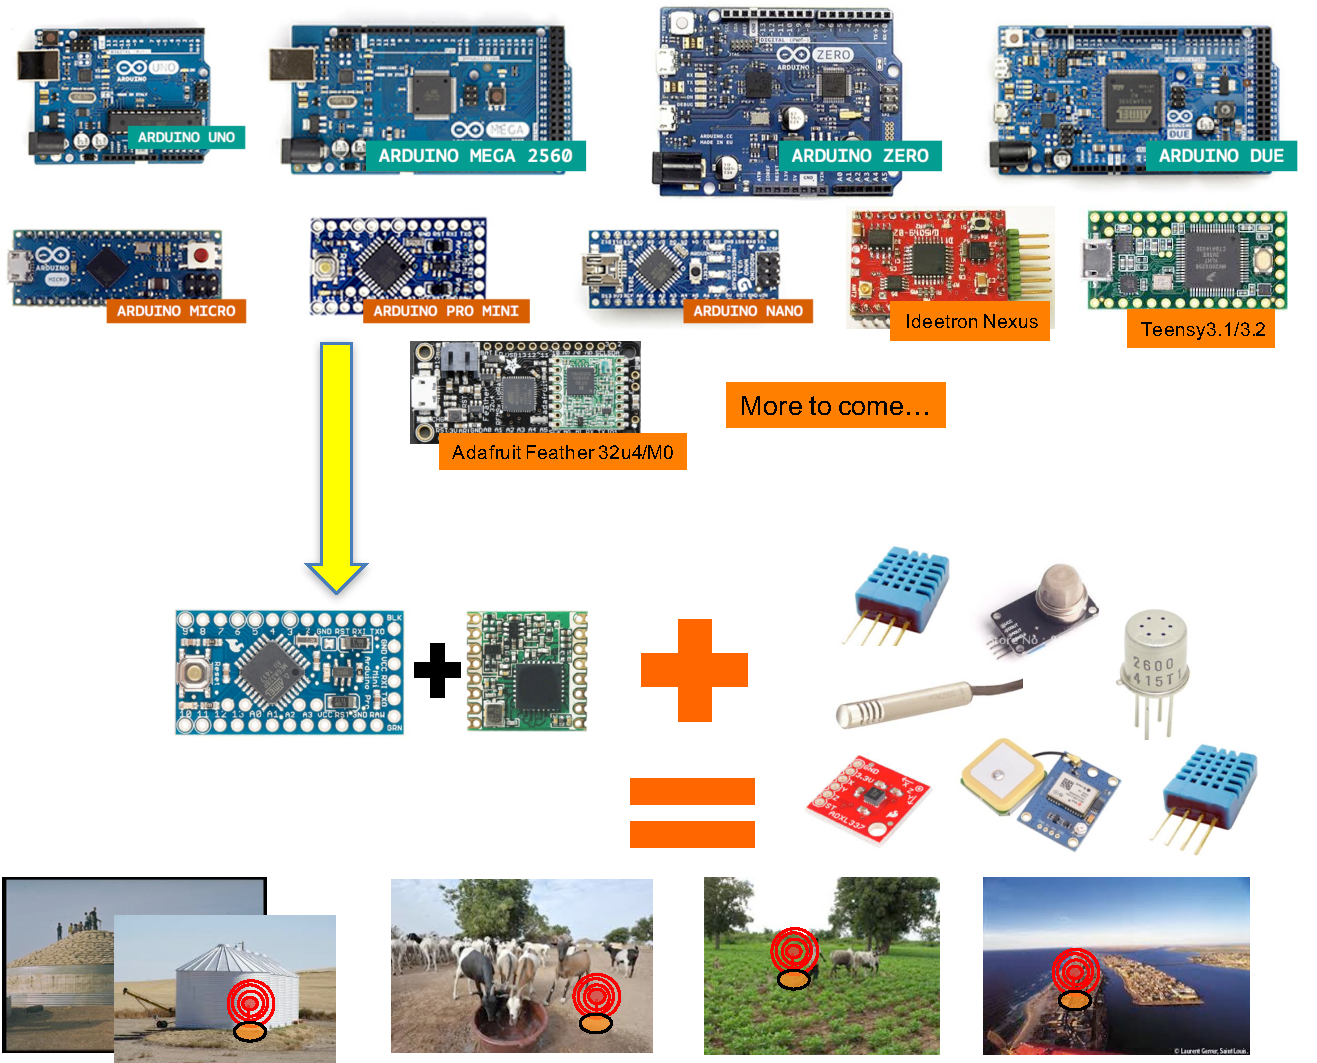
\includegraphics[width=.9\linewidth]{figures/generic-iot}   
  \label{figure-generic-iot}  
  \end{figure} 

\end{frame}

\begin{frame}
\frametitle{Easy integration}

About 7 euro: 2 euro for the Arduino (with ATmega328) and 5 euro for the radio module!
Arduino Pro Mini: 3.3v 8MHz running a year on 4 AA batteries
  \begin{figure}[H] 
  \centering  
  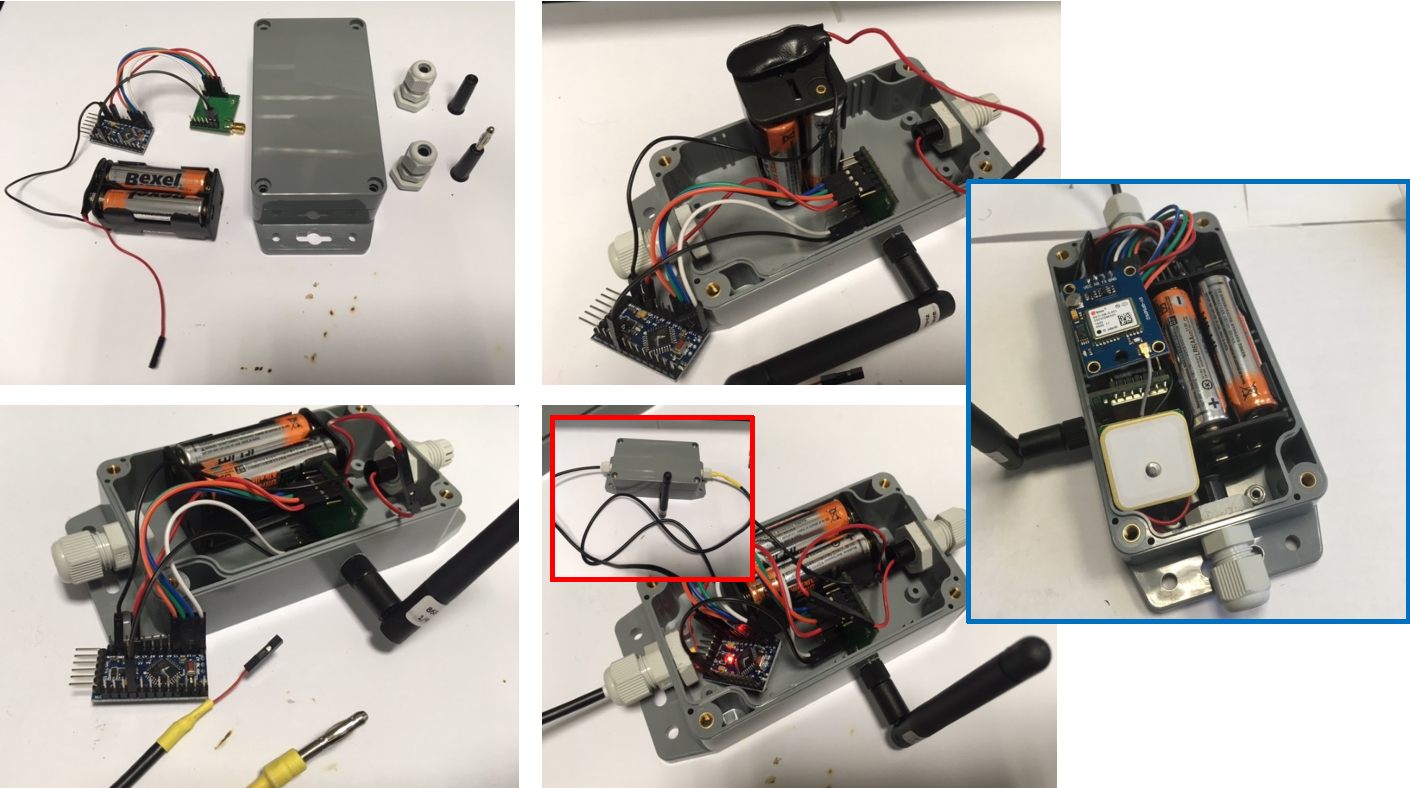
\includegraphics[width=.9\linewidth]{figures/easy-integration}   
  \label{figure-easy-integration}  
  \end{figure} 

\end{frame}

\section{Waziup Cloud platform}

\subsection{Architecture}

\begin{frame}
\frametitle{Architecture}

Waziup: a holistic IoT platform for Africa
  \begin{figure} 
  \centering  
  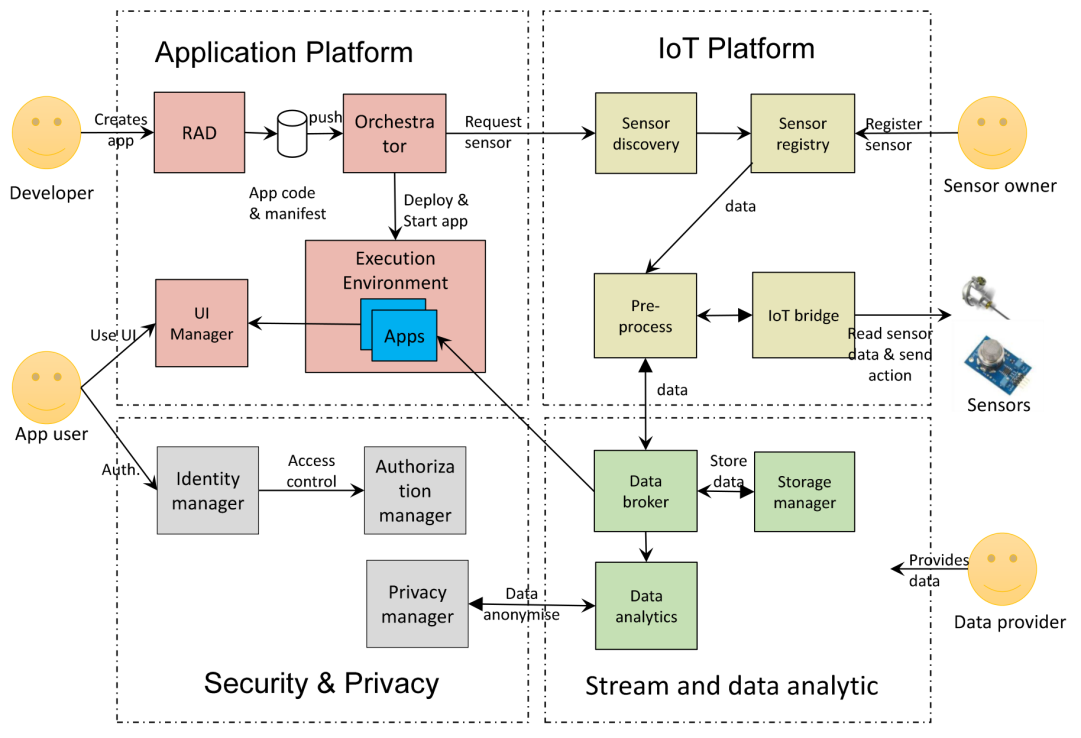
\includegraphics[width=.9\linewidth]{figures/GlobalArch}   
  \label{figure-globalarch}  
  \end{figure} 
  
\end{frame}

\begin{frame}
\frametitle{Local and global Clouds}

  Local cloud: installation of Waziup on a PC or directly on the gateway

  \begin{figure}[H] 
  \centering  
  \includegraphics[width=0.90\linewidth]{figures/localglobalcloud}   
  \label{fig-localglobalcloud}  
  \end{figure}
    
\end{frame}

\begin{frame}
\frametitle{API}

  \begin{table}
  \begin{tabular}{l | l }
    endpoint & methods \\
    \hline
    Sensors & GET, POST, PUT, DELETE \\ 
    Historical data & GET \\
    Farms & GET, POST, PUT, DELETE\\
    Notifications & GET, POST, PUT, DELETE \\
    Socials & GET, POST\\
    Users & GET, POST, PUT, DELETE \\
    Security & GET \\
    CEP & GET, POST, DELETE \\
    Apps & GET, POST, DELETE 
  \end{tabular}
  \end{table}
  
    
\end{frame}
\subsection{Security}

\begin{frame}
\frametitle{Authentication}
  
  \begin{itemize}
  \item Authentication: OpenID, OAuth tokens 
  \end{itemize}

  \begin{figure}
  \centering
  \includegraphics[width=1\linewidth]{figures/login.png}
  \end{figure}

\end{frame}

\begin{frame}
\frametitle{Authorization}
  
  \begin{itemize}
  \item Authorization: Role Based Access Control (RBAC)
  \end{itemize}

  \begin{figure}
  \centering
  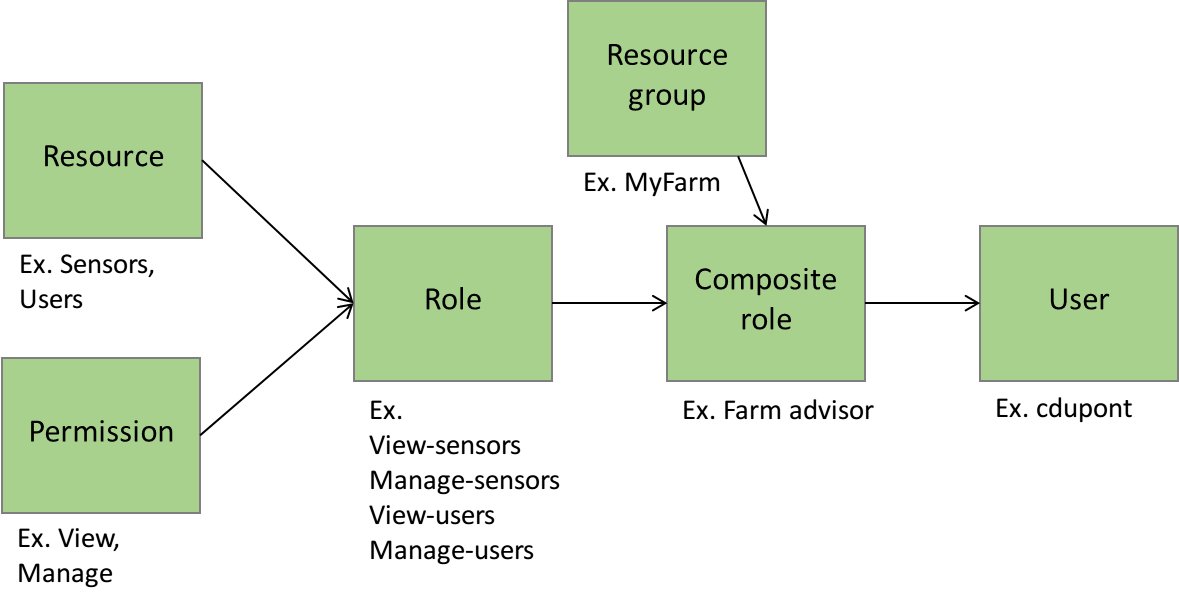
\includegraphics[width=.8\linewidth]{figures/RBAC.png}
  \end{figure}

\end{frame}
\subsection{Implementation}

\begin{frame}
\frametitle{Implementation}

  \begin{figure} 
  \centering  
  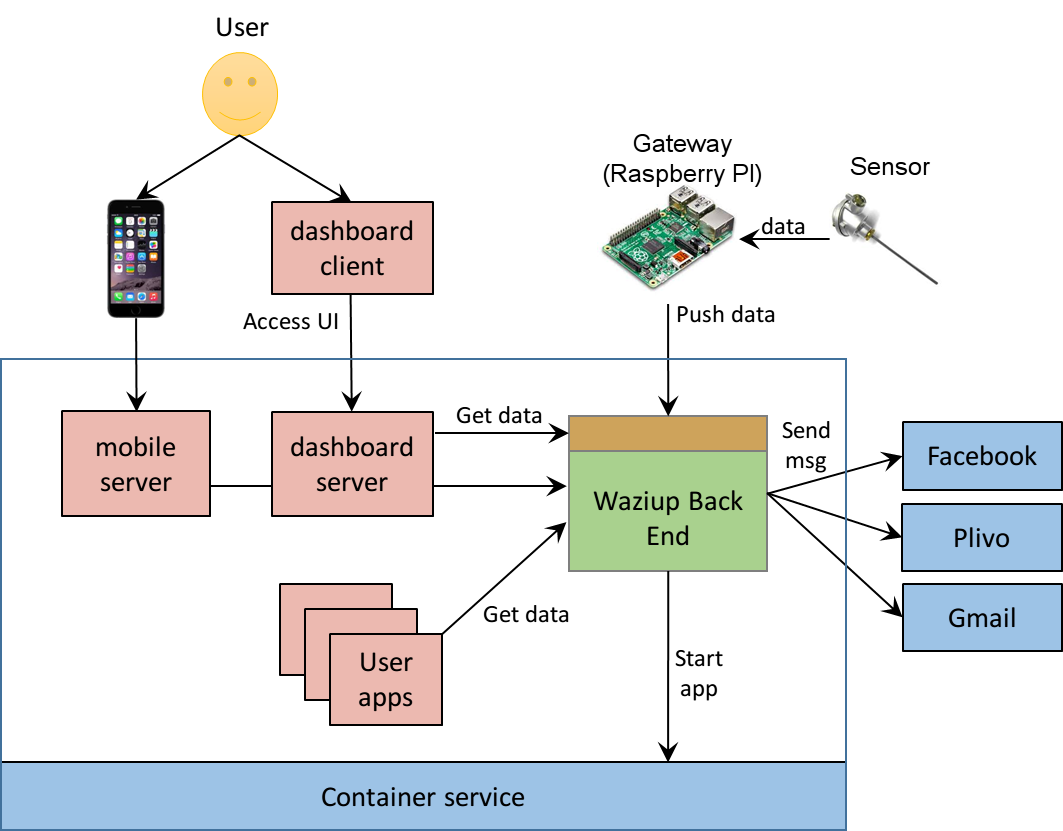
\includegraphics[width=.8\linewidth]{figures/CloudEnv.png}   
  \label{fig-implem}  
  \end{figure}

\end{frame}


\begin{frame}
\frametitle{Implementation}
 

  \begin{figure}
  \centering  
  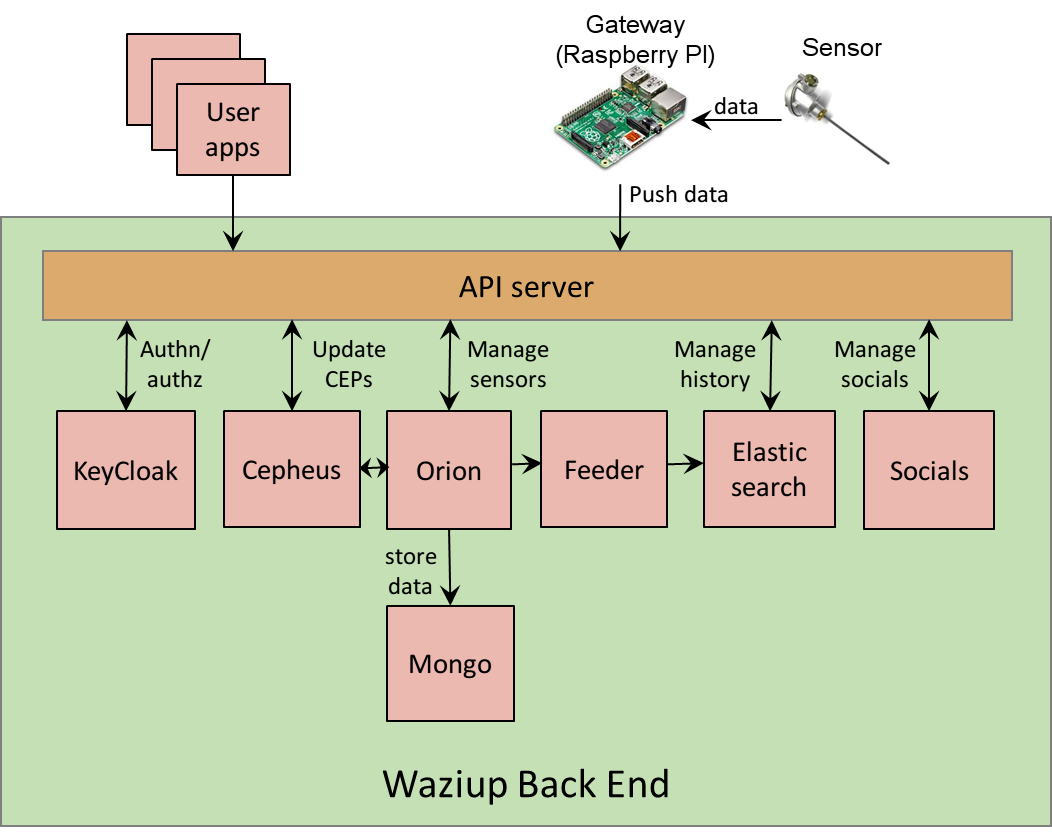
\includegraphics[width=.8\linewidth]{figures/BackEnd.png}   
  \label{fig-implem}  
  \end{figure}
\end{frame}

\begin{frame}
\frametitle{Data management \& analytics}

    
\end{frame}

\begin{frame}
\frametitle{Application platform}

  \begin{figure}[H]  
  \centering  
  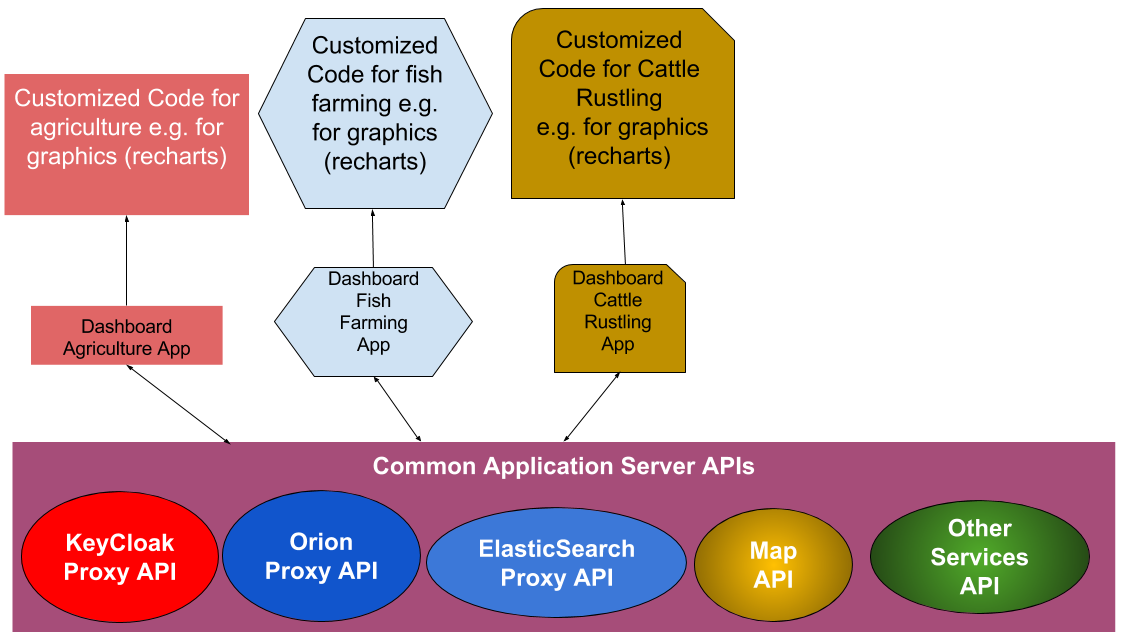
\includegraphics[width=.68\linewidth]{figures/AppArchitecture.png}   
  \caption{A global view of WAZIUP Application Template platform}
  \label{fig-app}
  \end{figure}
 
\end{frame}

\subsection{Dashboard}

\begin{frame}
\frametitle{Dashboard - sensors view}

  \begin{figure}[H]  
  \centering  
  \includegraphics[width=.73\linewidth]{figures/dashboard} 
  \label{fig-dashboard}
  \end{figure}

\end{frame}
  
\begin{frame}
\frametitle{Dashboard - graph view}

\vspace{-1cm}
  \begin{figure} 
  \centering  
  \includegraphics[width=.70\linewidth]{figures/sensor-data}
  \label{fig-sensor-data}
  \end{figure}
 
\end{frame}

\subsection{Service orchestration}


\begin{frame}
\frametitle{Service orchestration}

\end{frame}



\section{Conclusion}

\begin{frame}
\frametitle{Conclusion}
  
With ICT technologies, developing countries can dramatically improve its productivity by enabling the rapid and cost-effective deployment of advanced and real-time monitoring.
However, deploying an IoT platform in developing countries comes with many challenges.
Among them, the most important are supporting low cost, low power, low bandwidth, and intermittent Internet.

We presented:
  \begin{itemize}
    \item Hardware
    \item software Cloud platform 
  \end{itemize}

\end{frame}


\begin{frame}
\frametitle{Acknowledgements}

The authors would like to thank the EU H2020 projects Waziup, and the Create-Net FBK research centre. \\

\end{frame}

\end{document}
